\documentclass [12 pt, twoside] {article}

\usepackage[margin=1in]{geometry}
\usepackage[utf8]{inputenc}
\usepackage{listings}
\usepackage{color}
\usepackage{setspace}
\usepackage{graphicx}
\graphicspath{ {images/} }

\definecolor{codegreen}{rgb}{0,0.6,0}
\definecolor{codegray}{rgb}{0.5,0.5,0.5}
\definecolor{codeblue}{rgb}{0,0,0.6}
\definecolor{backcolor}{rgb}{0.95,0.95,0.95}

\lstdefinestyle{mystyle}{
	backgroundcolor = \color{backcolor},
	commentstyle = \color{codeblue},
	keywordstyle = \color{codegreen},
	numberstyle = \color{codegray},
	stringstyle = \color{magenta},
	basicstyle = \footnotesize,
	breakatwhitespace = false,
	breaklines = true,
	captionpos = b,
	keepspaces = true,
	numbers = left,
	numbersep = 5pt,
	showspaces = false,
	showstringspaces = false,
	showtabs = false,
	tabsize = 4
}

\lstset{style = mystyle}

\begin{document}

\title{Movement Code}
\author{Yicheng Wang}
\date{2014-11-20}
\maketitle

\section{Actual Code}
\begin{lstlisting}[language=C++]
void setPositionTarget(float target[3], float multiplier) {
	api.getMyZRState(me);
	
	float myPos[3],meMag;
	
	for(int i = 0; i < 3; i++) {
		myPos[i] = me[i];
	}
	
	meMag = mathVecMagnitude(myPos,3);
	
	if (minDistanceFromOrigin(target) > 0.31) {
		if (distance(me, target) < 0.4) { // Save braking distance
			api.setPositionTarget(target);
		}

		else { // Or haul ass towards target
			float temp[3];

			mathVecSubtract(temp,target,me,3);
			
			for (int i = 0 ; i < 3 ; i++) {
				temp[i] = me[i] + temp[i] * multiplier;
			}

			api.setPositionTarget(temp);
		}

		DEBUG(("GOING STRAIGHT\n"));
	}
	
	else if (meMag >= 0.22 && meMag <= 0.32) {
		for (int i = 0; i < 3; i++) {
			myPos[i] = myPos[i] * 1.6;
		}
		
		api.setPositionTarget(myPos);
		DEBUG(("TOO CLOSE\n"));
	}
	
	else {
		float opposite[3], perpendicular[3], mePrep[3], path[3], temp[3];
		
		mathVecProject(opposite,target,myPos,3);
		mathVecSubtract(perpendicular,target,opposite,3);
		
		for (int i = 0; i < 3; i++) {
		    mePrep[i] = perpendicular[i] / mathVecMagnitude(perpendicular,3);
		}
		
		for (int i = 0; i < 3; i++) {
			mePrep[i] = (mePrep[i] * 0.325 * meMag) / (sqrtf(meMag*meMag - 0.32*0.32));
		}
		
		mathVecSubtract(path,mePrep,myPos,3);
		
		for (int i = 0; i < 3; i++) {
			path[i] = path[i] * multiplier;
		}
		
		mathVecAdd(temp,myPos,path,3);

		api.setPositionTarget(temp);
		
		DEBUG(("TAKING THE TANGENT\n"));
	}
}

void mathVecProject(float c[], float a[], float b[], int n) {
    // finds the projection of a onto b, puts the result in c
    for (int i = 0; i < n; i++) {
        c[i] = (mathVecInner(a,b,3) * b[i]) / (mathVecMagnitude(b,3) * mathVecMagnitude(b,3));
    }
}

float minDistanceFromOrigin(float target[]) {
	ZRState me;
	float path1[3], path2[3], dot, cosine;
	
	mathVecSubtract(path1,target,me,3);
	mathVecSubtract(path2,me,target,3);
	
	dot = mathVecInner(path1,me,3);
	
	cosine = dot / (mathVecMagnitude(path1, 3) * mathVecMagnitude(me, 3));
	
	if (cosine < 0) {
		return mathVecMagnitude(me, 3);
	}
	
	dot = mathVecInner(path2,target,3);
	
	cosine = dot / (mathVecMagnitude(path2, 3) * mathVecMagnitude(target, 3));
	
	if (cosine < 0) {
		return mathVecMagnitude(target,3);
	}
	
	else {
		float dis[3], negMe[3];
		
		mathVecSubtract(path1,target,me,3);
		
		for(int i = 0; i < 3; i++) {
			negMe[i] = -me[i];
		}
		
		mathVecProject(path2,negMe,path1,3);
		
		mathVecAdd(dis,me,path2,3);
		
		return mathVecMagnitude(dis,3);
	}
}
\end{lstlisting}

\section{Basic Idea}


\indent The idea here is that we can shoot for the target position as long as you don’t collide with the
asteroid on your trajectory. A simple vector diagram for definition purposes is presented in Figure 1.


A simple explanation is also presented below:


We want to get a clear shot from the sphere’s position (MyPos) to the target position
(Target), both of which are represented as vectors. Our goal is to travel to the target without coming in contact with the asteroid. The way to do this is to find the two tangents to the asteroid.
The way to find the second tangent is easy; as soon as the sphere gets a clear shot, it’ll travel
straight to the target (line 12-30 of the code). Before then, however, things are a bit complicated.
To do this, we first project the Target vector onto MyPos, which creates the vector called
Opposite. Then, we subtract that vector from Target to create Perpendicular, which is perpendicular
to the MyPos vector, and is within the plane formed by the Target vector and MyPos vector. Now we 
just have to find its length so that it is tangent to the asteroid (or danger zone sphere). To do so, we draw similar triangles! Suppose
the desirable distance such that the tangent path is x; we draw the radius to the point of
tangency. We know that this radius is perpendicular to the hypotenuse formed by MyPos and x.
By some trival geometry, we can tell that the triangle formed by the radius, MyPos and the origin
is similar to the triangle formed by MyPos, x and the origin. Now, we set the length in ratio:
$$\sqrt{(||MyPos||)^2 - r^2} : r = ||MyPos|| : x$$
So we get:
$$x = \frac{r \cdot ||MyPos||}{\sqrt{(||MyPos||)^2 - r^2}}$$
Hence line 52 of the code.

\begin{figure}[h]
\centering
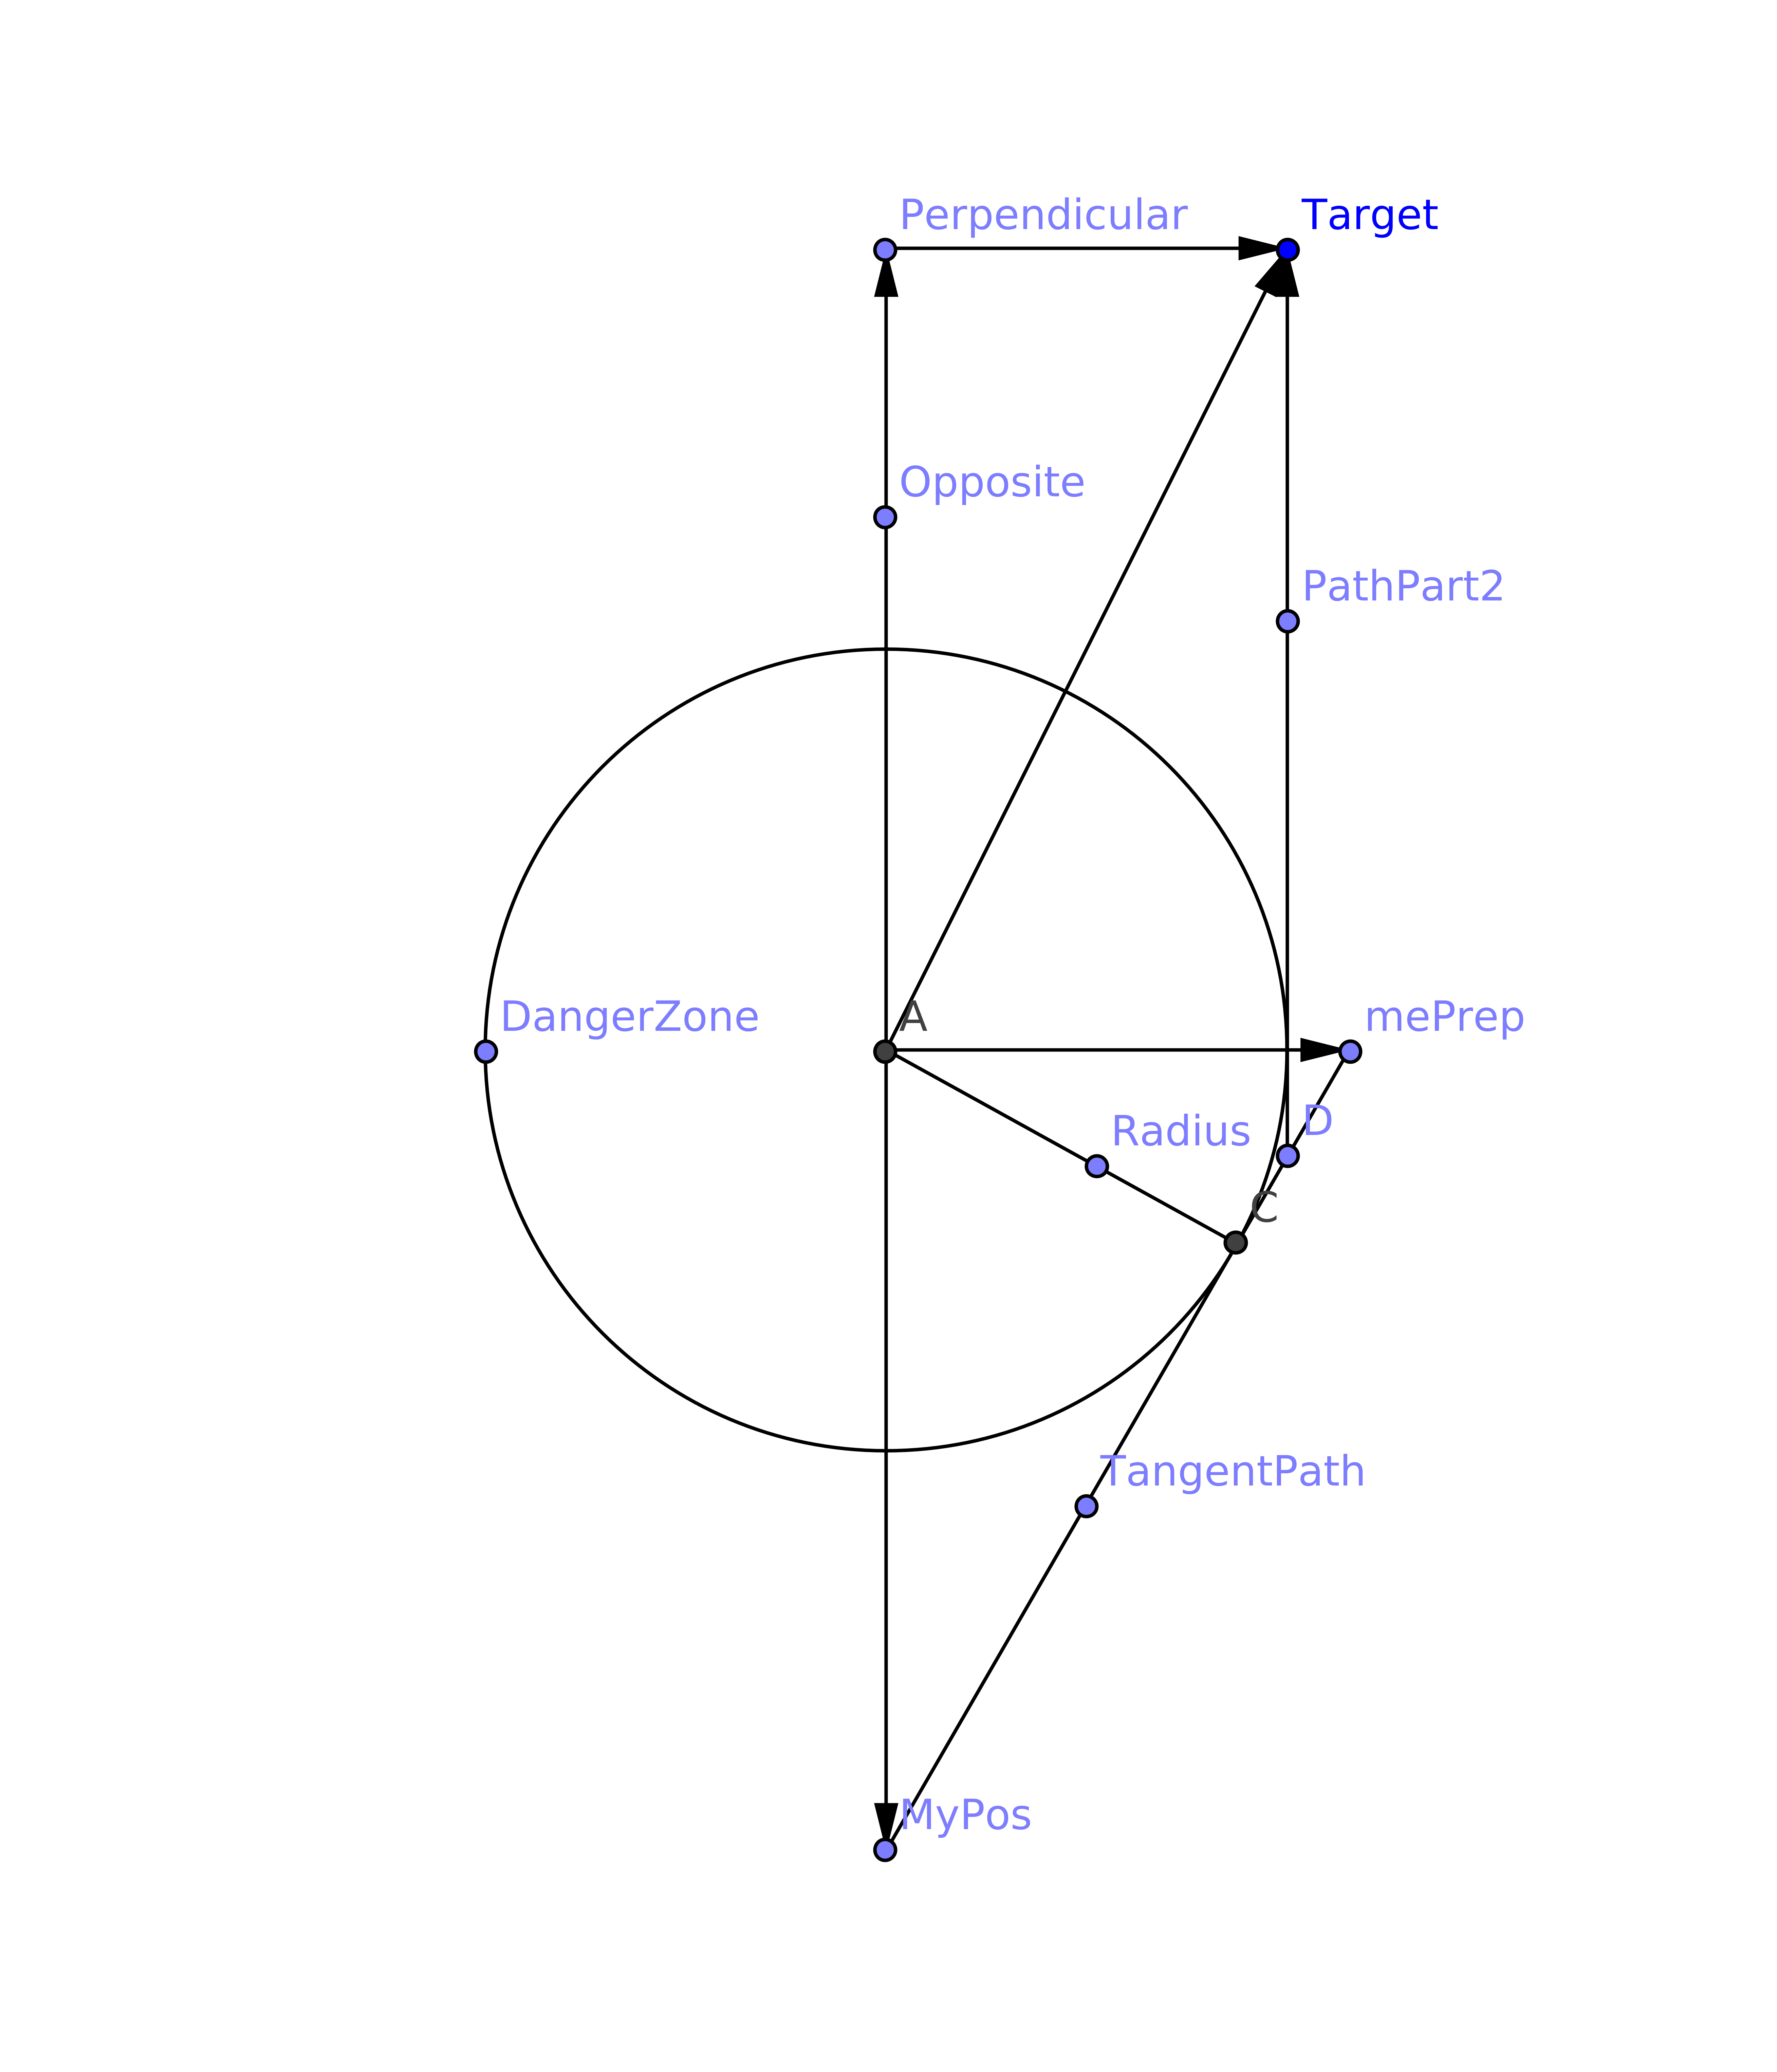
\includegraphics[scale=0.2]{setPositionTarget.png}
\caption{Diagram for setPositionTarget}
\end{figure}




The rest are really error handeling and those are pretty simple to understand.


\section{Increased Efficiency via Phantom Target Creation}


\indent The API function setPositionTarget may be annoying to use in that it slows down upon
reaching its target. However, sometimes that's bad when you don't need to stablize, like
phase 1 (tangent phase) of the movement function. This can be solved by creating a Phantom
target that is a direct multipler of where you want to go, so that when the api function
sees that the sphere is nowhere near this phantom target, it'll keep accelerating and make
the sphere run very fast, as exemplified by line 23 and 58 of the code.


However, this method should be used with caution and MAKE SURE that you can and will break
out of the phantom target loop before it goes too far. Note that there is a braking distance
built into the function, but for high multipliers (like 9), it becomes hard to control
and will easily hurl the sphere out of bounds (or into the asteorid).

\end{document}
